\subsection{Inteligencia Artificial}

El método racional combina la ingeniería y las matemáticas en base a las "leyes del pensamiento", que se remontan a la antigua Grecia y son influenciadas por filósofos como Aristóteles. Se desarrollaron programas capaces de resolver problemas de lógica en el siglo XIX. Por lo tanto, el objetivo de la inteligencia artificial en el mundo real es desarrollar sistemas inteligentes que tengan estas capacidades. Incluso cuando hay incertidumbre, un "agente racional" actúa para lograr el mejor resultado posible. La inteligencia artificial se basa en una variedad de ciencias, como la ingeniería computacional, la teoría de control, la cibernética, la lingüística, la filosofía, la economía, la psicología, la neurociencia y las matemáticas, según \parencite{bk_russell2004intart}.

Dos investigadores en neurociencia crearon el primer modelo de IA basado en neuronas artificiales en 1943, dando inicio al análisis de la inteligencia artificial. Warren McCulloch y Walter Pitts idearon un modelo que permitía que las neuronas fueran "activadas" o "desactivadas", lo que demostró que una red de neuronas era capaz de realizar cualquier tarea computacional. Posteriormente, Donald Hebb propuso la "regla de aprendizaje hebbiano". John McCarthy, Allen Newell y Herbert Simon desarrollaron un programa capaz de pensar de forma no numérica en el taller de Dartmouth, aunque no se publicó. El término "Inteligencia Artificial" fue acuñado por McCarthy, \parencite{bk_russell2004intart}.

La IA comenzó a entrar en la industria en los años 80, especialmente en grandes empresas de países desarrollados, a través de la investigación en sistemas expertos y el desarrollo de computadoras más poderosas.

Hoy en día, la inteligencia artificial tiene una amplia gama de aplicaciones, incluida la minería de datos, el procesamiento de lenguaje natural, la robótica y los videojuegos, junto con subdominios como el aprendizaje automático y la visión computacional.

\subsection{Aprendizaje Automático}
El aprendizaje automático es una rama de la inteligencia artificial que se centra en técnicas que permiten a las computadoras aprender mediante algoritmos y heurísticas, transformando muestras de datos en programas sin necesidad de programación explícita. \parencite{bk_russell2009intart} describen el aprendizaje automático como una rama de la inteligencia artificial. Estos algoritmos utilizan tecnologías como el procesamiento del lenguaje natural, el aprendizaje profundo y las redes neuronales. Ambos tipos de aprendizaje, supervisado y no supervisado, se basan en lecciones derivadas de datos. El desarrollo de algoritmos que puedan recibir datos de entrada y utilizar análisis estadístico para predecir una salida, que cambia a medida que se adquieren nuevos datos, es la base del aprendizaje automático. \parencite{bk_alpaydin2014ml}

Se puede clasificar en cuatro tipos principales de la siguiente manera según el objetivo que se desea alcanzar mediante el uso de ML:
\begin{itemize}
	\item \textbf{Aprendizaje supervisado}: El aprendizaje supervisado se ganó su nombre porque los científicos de datos actúan como una guía para enseñarle al algoritmo las conclusiones a las que debe llegar. Es similar a la forma en que un estudiante aprende aritmética básica de un maestro. Este tipo de aprendizaje requiere datos etiquetados con las respuestas correctas que se esperan del resultado del algoritmo. Para problemas de clasificación y regresión, el aprendizaje supervisado demostró ser preciso y rápido según \parencite{bk_zambrano2018supnosup}.
	
	Los dos tipos de aprendizaje supervisado son:

	\begin{itemize}
		\item \textbf{La Clasificación}: es la predicción del valor categórico de salida que permite dividir los datos en clases específicas. La clasificación se puede usar para varios propósitos, como determinar el clima, determinar si un correo electrónico es spam o no o identificar tipos de animales después de recibir una educación adecuada, un conjunto de datos con etiquetas de imágenes que incluyen la especie y algunas identificaciones características, según \parencite{bk_zambrano2018supnosup}.
		\item \textbf{La Regresión}: es un tipo de problema en el que la predicción de un valor de respuesta continua es necesaria, como los precios de las acciones y la vivienda, según \parencite{bk_zambrano2018supnosup}.
	\end{itemize}

	Por lo tanto, funciona modelando las relaciones y dependencias entre las características de entrada y la salida de predicción objetivo, lo que permite predecir los valores de salida para nuevos datos utilizando las relaciones que aprendió de conjuntos de datos anteriores, según \parencite{bk_alpaydin2014ml}.

	\item \textbf{Aprendizaje no supervisado}: Por otro lado, el aprendizaje no supervisado se asemeja más a lo que algunos expertos llaman inteligencia artificial real: la idea de que una máquina puede aprender a identificar patrones y procesos complejos sin la supervisión de humanos. Cuando los expertos no saben qué buscar en los datos y los datos en sí no incluyen objetivos, este método es particularmente útil. La agrupación de k-means, el análisis de componentes principales e independientes y las reglas de asociación según \parencite{bk_zambrano2018supnosup} son algunos de los muchos casos de uso del aprendizaje automático no supervisado.
	
	\begin{itemize}
		\item \textbf{Agrupación K-means}: es un tipo de problema en el que cosas similares están agrupadas, como se muestra en la Figura 16. Comparte el mismo concepto con la clasificación, pero no se proporcionan etiquetas, por lo que el sistema entenderá los datos y los agrupará. Un uso de esto sería agrupar los artículos y las noticias según su género y contenido, según \parencite{tec_sancho2018supnosup}
	\end{itemize}
	
		\begin{figure}[h]
		\begin{center}
			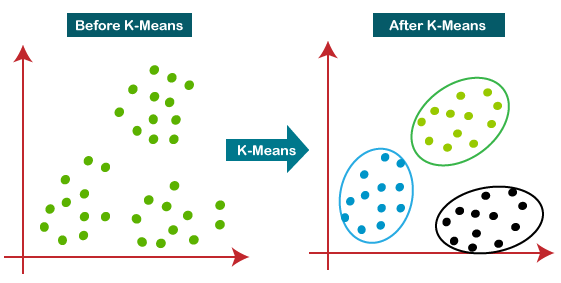
\includegraphics[width=0.75\textwidth]{2/figures/kmeans.png}
			\caption[Funcionamiento del algoritmo de K medias]{Funcionamiento del algoritmo de K medias.\\
			Fuente: \cite{tec_sancho2018supnosup}. \citetitle{tec_sancho2018supnosup}.}
			\label{2:fig3}
		\end{center}
	\end{figure}
		
	Debido a su complejidad y dificultad de implementación, este tipo de aprendizaje automático no se utiliza tan frecuentemente como el aprendizaje supervisado, a pesar de que abre las puertas a la resolución de problemas que los humanos normalmente no abordarían, según \parencite{tec_sancho2018supnosup}

	\item \textbf{Aprendizaje semisupervisado}: Hasta el momento, todos los datos enviados han sido etiquetados con el resultado deseado o no han sido etiquetados en absoluto. El aprendizaje automático semisupervisado utiliza ambos. El costo de etiquetar es bastante alto en muchas situaciones prácticas y, en el caso de grandes conjuntos de datos, se vuelve aburrido y requiere mucho tiempo. Además, proporcionar demasiados datos etiquetados puede hacer que el modelo tenga sesgos humanos. A pesar de que los datos sin etiquetar son desconocidos para la red, ofrecen información útil sobre los parámetros del grupo objetivo. que conduce a la conclusión de que se puede mejorar la precisión del modelo al incluir datos sin etiquetar y, al mismo tiempo, ahorrar tiempo y dinero en su construcción. Por ejemplo, la clasificación de páginas web, el reconocimiento de voz o la secuenciación genética pueden usar aprendizaje automático semisupervisado. En esos casos, los científicos de datos pueden acceder a grandes cantidades de datos sin etiquetarlos, y la tarea de etiquetarlos todos llevaría mucho tiempo, según \parencite{bk_zambrano2018supnosup}.

	Se puede comparar estos tres tipos de aprendizaje automático para el mismo uso, como clasificación, utilizando los datos recopilados hasta ahora:

	\begin{itemize}
		\item \textbf{Clasificación supervisada}: el algoritmo clasificará los tipos de páginas web según las etiquetas proporcionadas desde el principio, según \parencite{bk_zambrano2018supnosup}.
		\item \textbf{Agrupación no supervisada}: el algoritmo buscará patrones y características que ayudan a agrupar páginas web en grupos, según \parencite{bk_zambrano2018supnosup}.
		\item \textbf{Clasificación semi no supervisada}: identificará varios grupos de páginas web utilizando los datos etiquetados, luego utilizará los datos no etiquetados para establecer los límites de esos grupos de páginas web y buscar otros tipos que posiblemente no aparezcan en los datos etiquetados, según \parencite{bk_zambrano2018supnosup}.
	\end{itemize}
	

	\item \textbf{Aprendizaje por refuerzo}: junto con el aprendizaje supervisado y no supervisado, es el aprendizaje por refuerzo. Como se muestra en la Figura 17, se compone de cinco componentes principales: el agente, el entorno, el estado, la acción y la recompensa. Utilizando su interacción con el entorno, RL busca maximizar la recompensa y reducir el riesgo. El algoritmo RL (también conocido como agente) mejorará el entorno a intervalos regulares experimentando varios estados potenciales. Los agentes seleccionarán automáticamente el comportamiento ideal para maximizar el rendimiento. La retroalimentación, también conocida como recompensa, es lo que permite al agente mejorar su comportamiento, según \parencite{bk_sutton2018rl}.
	
	\begin{figure}[h]
		\begin{center}
			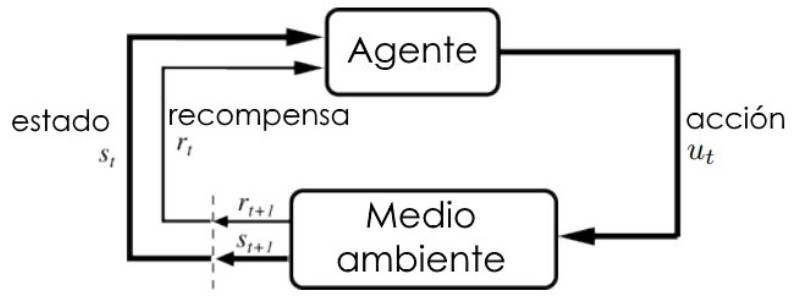
\includegraphics[width=0.60\textwidth]{2/figures/aprendizaje_refuerzo.jpg}
			\caption[Componentes del Aprendizaje por Refuerzo]{Componentes del Aprendizaje por Refuerzo.\\
				Fuente: \cite{bk_sutton2018rl}. \textit{Finite Markov Decision Processes}. (p. 48)}
			\label{2:fig4}
		\end{center}
	\end{figure}
	
\end{itemize}

\subsection{Aprendizaje Profundo}

Desde que llegó la Inteligencia Artificial hace un tiempo, tiene una amplia gama de aplicaciones y se divide en muchas ramas, como se menciona en \parencite{gl_sas_deeplearning}. El aprendizaje profundo es un subconjunto del aprendizaje automático, que es en sí mismo un subcampo de la IA. La Figura 18 es una representación visual de la relación entre AI, ML y DL.

\begin{figure}[!ht]
	\begin{center}
		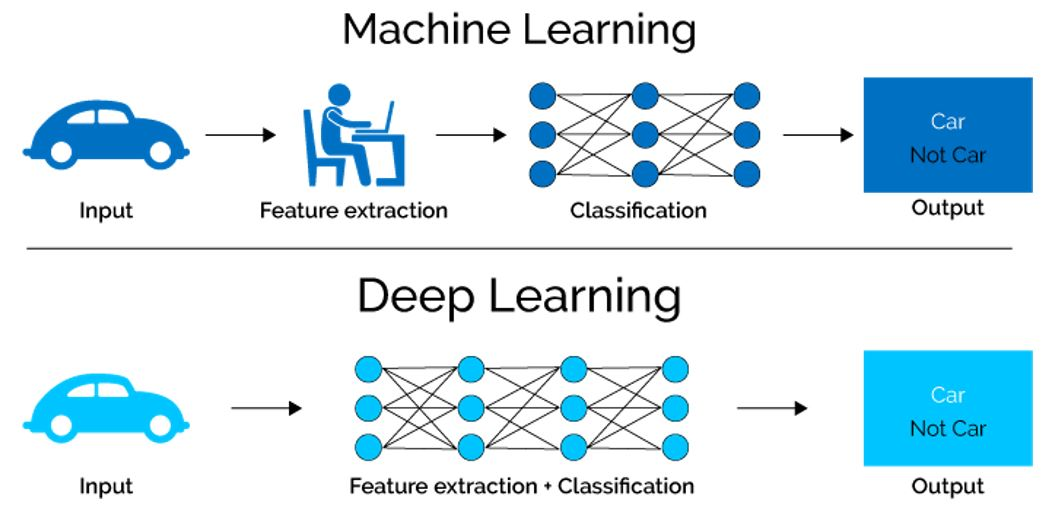
\includegraphics[width=0.50\textwidth]{2/figures/deeplearning_machinelearning.jpg}
		\caption[Relación entre IA, ML y DL]{Relación entre IA, ML y DL.\\
		Fuente: \cite{tec_cook2018deeplearning}. \textit{Most Popular 20 Free Online Courses to Learn Deep Learning}.}
		\label{2:fig5}
	\end{center}
\end{figure}

El aprendizaje profundo no solo permite representar datos de la manera correcta, sino que también permite que la computadora aprenda programas informáticos de varios pasos al incluir el concepto de profundidad en sus modelos. Como se muestra en la Figura 19, cada capa de representación puede interpretarse como el estado de la memoria de la computadora. Las computadoras interpretan las imágenes como una colección de valores de píxeles que representan escenas de nuestra realidad. Según \parencite{tec_cook2018deeplearning}, identificar un objeto o mapear su identidad a partir de esos valores es una tarea difícil para las máquinas y puede resultar casi imposible cuando se intenta aprender este mapeo directamente.

\begin{figure}[!ht]
	\begin{center}
		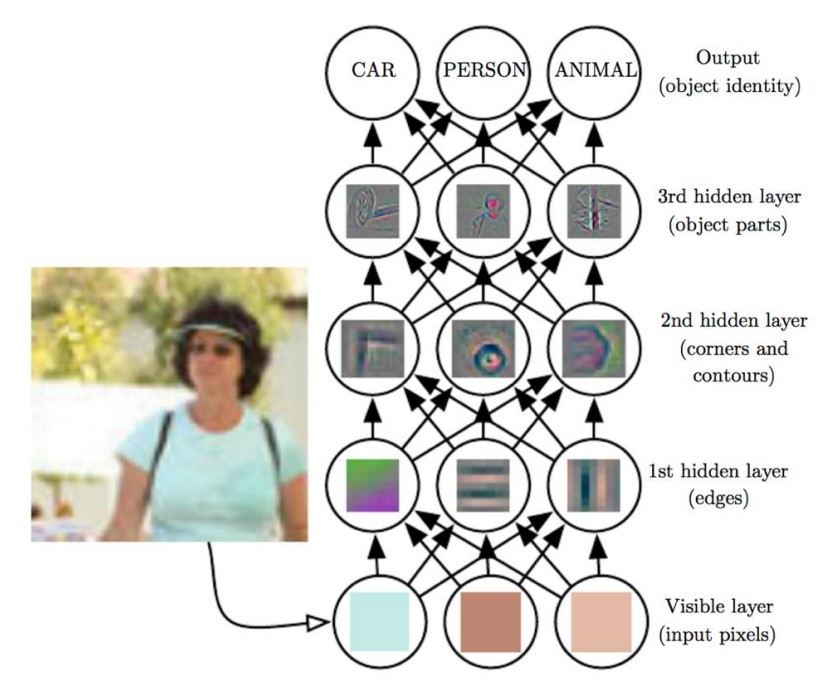
\includegraphics[width=0.70\textwidth]{2/figures/deeplearning_machinelearning2.jpg}
		\caption[Ilustración de un modelo de aprendizaje profundo]{Ilustración de un modelo de aprendizaje profundo.\\
		Fuente: \cite{tec_cook2018deeplearning}. \textit{Most Popular 20 Free Online Courses to Learn Deep Learning}.}
		\label{2:fig6}
	\end{center}
\end{figure}


\subsection{Aprendizaje Profundo Multimodal}
Como se muestra en la Figura \ref{2}, el fundamento del aprendizaje profundo multimodal es la integración de diversas modalidades (como audio, imágenes, texto, videos, etc.) o múltiples tareas (como predicción, clasificación, series de tiempo, etc.) a través del uso de representaciones latentes en redes neuronales profundas. \parencite{bk_deng2018deeplearningnlp}.

\begin{figure}[!ht]
	\begin{center}
		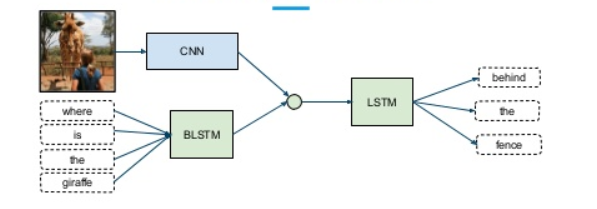
\includegraphics[width=0.85\textwidth]{2/figures/multimodal_network.png}
		\caption[Un modelo multimodal que combina imágenes y texto]{Un modelo multimodal que combina imágenes y texto.\\
		Fuente: \cite{tec_nishida2015multimodal}. \textit{Multimodal gesture recognition using multi-stream recurrent neural network}.}
		\label{2:fig7}
	\end{center}
\end{figure}

Este tipo de modelos pueden realizar inferencias más robustas porque las señales de diferentes modalidades proporcionan información complementaria sobre distintos aspectos de un objeto, evento o actividad. Las técnicas multimodales, como la fusión temprana y tardía, la fusión de modelos, el ensamblaje de modelos y las redes neuronales profundas, se utilizan actualmente. Los "enfoques aditivos" facilitan la realización de predicciones al combinar características para la toma de decisiones y la recopilación de información útil, según \parencite{tec_liu2018multideeplearning}.

\cite{tec_baheti2020introduction_mdl} afirman que el uso de modelos multimodales mejora el rendimiento de las redes neuronales y permite una extracción más efectiva de características de todas las fuentes, lo que favorece predicciones a mayor escala. Uno de los principales beneficios es que los datos de diferentes fuentes ofrecen información complementaria que revela patrones ocultos que no se pueden ver cuando las modalidades se analizan individualmente, mejorando así la precisión de las predicciones.

\begin{figure}[!ht]
	\begin{center}
		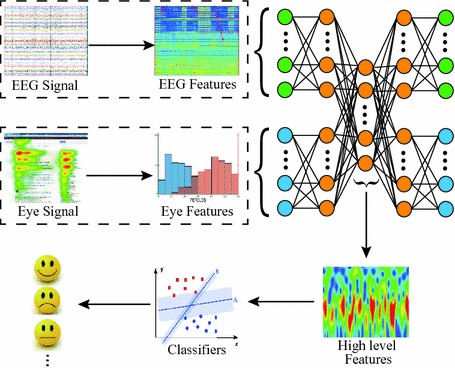
\includegraphics[width=0.79\textwidth]{2/figures/multimodal_deep_learning_example.jpg}
		\caption[Un modelo multimodal para las señales de electroencefalografía y de ojo]{Un modelo multimodal para las señales de electroencefalografía y de ojo.\\
		Fuente: \cite{tec_baheti2020introduction_mdl}. \textit{Introduction to Multimodal Deep Learning}.}
		\label{2:fig7}
	\end{center}
\end{figure}

\subsection{Inteligencia Artificial Generativa}

La inteligencia artificial generativa es el campo de la ciencia que estudia cómo crear inteligencia totalmente automatizada. Esto contrasta con el campo de la inteligencia artificial moderna, que investiga cómo los humanos comprenden y construyen la inteligencia. La construcción manual es lo que hacen los investigadores, pero la parte "por humanos" de la definición de IA suele ser una variable oculta en la construcción de los sistemas de IA contemporáneos. Aunque la diferencia puede parecer sutil, incluso innecesaria, la construcción automatizada requiere una perspectiva completamente nueva, que no está disponible en la literatura sobre IA actual. No importa si los humanos comprenden cómo funcionan los mecanismos internos de una máquina en la Inteligencia Artificial Generativa, aunque podría ayudar a los investigadores en su búsqueda de la creación de máquinas inteligentes. Lo que importa es que la máquina pueda controlar y dirigir el proceso de creación de estructuras internas en la dirección deseada. Es como criar hijos: los seres humanos no son conscientes de los procesos mentales, pero interactúan con sus hijos en un nivel diferente al hablar de sus sustratos neuronales. En lugar de eso, utilizan una variedad de máquinas clasificadoras para diferenciar los comportamientos positivos de los negativos, que podrían ser beneficiosos para el niño cuando sea mayor. Los castigos corporales, los institutos educativos, los medios de comunicación y otros lugares son algunos de los usos de estas máquinas clasificadoras, según \parencite{th_zant2010genai}

A continuación, ofrecemos una variedad de categorías de modelos de inteligencia artificial generativa.

\begin{itemize}
	\item \textbf{Modelos de difusión}: crean nuevos datos iterando cambios aleatorios controlados en una muestra de datos previa. Empezan con los datos originales y luego agregan cambios sutiles, también conocidos como ruido, que hacen que gradualmente pierdan la similitud con el original. Este ruido se controla minuciosamente para garantizar que los datos generados sigan siendo consistentes y realistas. El modelo de difusión invierte el proceso después de agregar ruido en varias iteraciones. Como se muestra en la Figura 22, la eliminación de ruido inversa crea una muestra de datos nueva que se asemeja a la original, según \parencite{tec_amaz2023iagen}.
	
	\begin{figure}[!ht]
		\begin{center}
			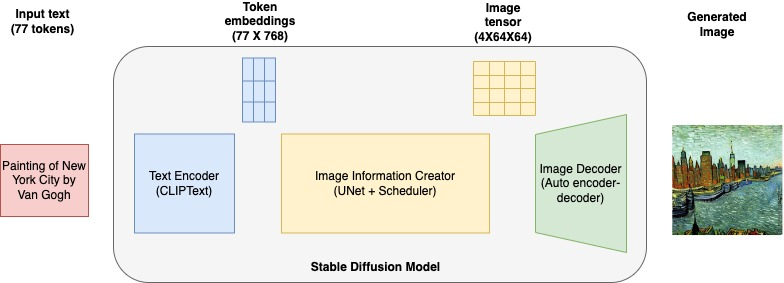
\includegraphics[width=0.85\textwidth]{2/figures/modelosdedifusion.jpg}
			\caption[Modelos de difusión]{Modelos de difusión.\\
			Fuente: \cite{tec_amaz2023iagen}. \citetitle{tec_amaz2023iagen}.}
			\label{2:fig8}
		\end{center}
	\end{figure}

	\item \textbf{Redes generativas adversativas}: compiten con dos redes neuronales. La primera red, también conocida como generador, agrega ruido aleatorio para crear muestras de datos falsas. La segunda red, conocida como discriminador, ayuda a distinguir entre los datos reales y falsos generados por el generador. El generador mejora continuamente su capacidad de generar datos realistas, mientras que el discriminador mejora su capacidad de distinguir entre lo real y lo falso. Hasta que el generador produzca datos tan persuasivos que el discriminador no pueda diferenciarlos de los datos reales, este proceso adversativo termina, según \parencite{tec_amaz2023iagen}.

	\item \textbf{Autocodificadores variacionales}: aprenden sobre el espacio latente, una pequeña representación de datos. La representación matemática de los datos se conoce como espacio latente. Puede verse como un código único que representa los datos en función de cada característica. Por ejemplo, cuando se estudian los rostros, el espacio latente contiene números que representan la forma de las orejas, los pómulos, la nariz y los ojos. Las dos redes neuronales utilizadas por los VAE son el codificador y el decodificador. Para cada dimensión del espacio latente, la red neuronal del codificador mapea los datos de entrada a una media y una varianza. crea una muestra aleatoria utilizando la distribución normal gaussiana. Este ejemplo es un punto en el espacio latente, y como se puede ver en la Figura 23, representa una versión comprimida y simplificada de los datos de entrada, según \parencite{tec_amaz2023iagen}.
	
	\begin{figure}[!ht]
		\begin{center}
			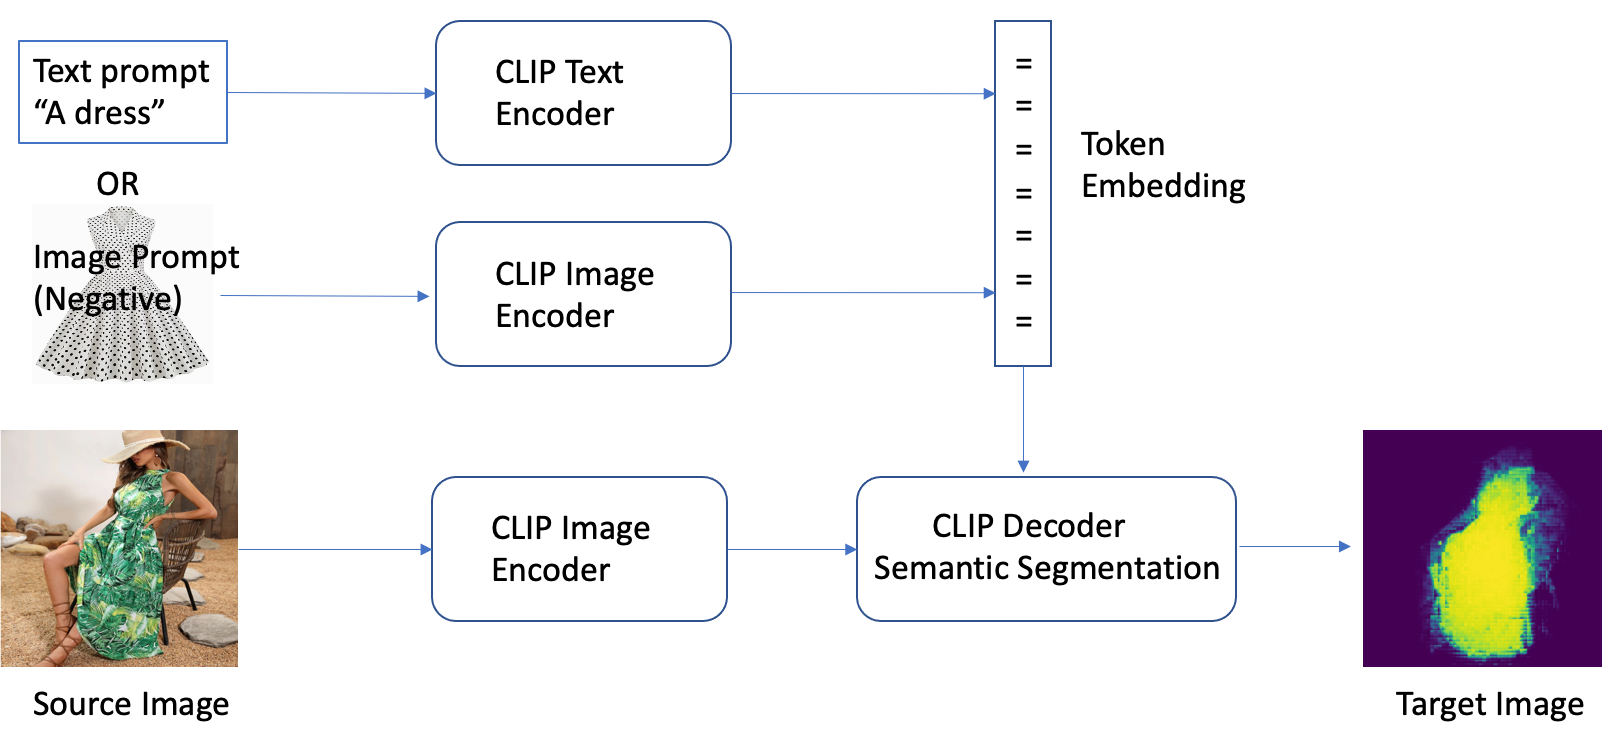
\includegraphics[width=0.85\textwidth]{2/figures/autocodificadoresvariacionales.png}
			\caption[Autocodificadores variacionales]{Autocodificadores variacionales.\\
			Fuente: \cite{tec_amaz2023iagen}. \citetitle{tec_amaz2023iagen}.}
			\label{2:fig9}
		\end{center}
	\end{figure}
\end{itemize}


\subsection{Modelos de Predicción}

Los modelos estadísticos se utilizan para prever comportamientos futuros mediante la recopilación de datos actuales e históricos, la creación de modelos estadísticos, la realización de predicciones y la validación continua a medida que se recopilan más datos. Estos modelos predictivos identifican patrones ocultos y usan el rendimiento pasado para calcular la probabilidad de que un agente presente un comportamiento específico en el futuro. \parencite{gl_gartner2019pm}

\subsection{Análisis de Datos Espaciales}

El análisis espacial es una colección de técnicas y modelos que utilizan explícitamente referencias espaciales para cada valor de datos u objeto especificado en el sistema en estudio. Los métodos de análisis espacial necesitan hacer suposiciones o basarse en datos para describir las relaciones espaciales o interacciones espaciales entre casos. Los resultados de cualquier análisis espacial no son iguales cuando se reordenan la distribución espacial de valores o se reconfigura la estructura espacial del sistema. \parencite{bk_haining2003spdat}

Al realizar un análisis estadístico, es necesario tener en cuenta muchas características de los datos espaciales. El análisis de la dependencia espacial es crucial para el análisis de datos espaciales y central, por ejemplo, para realizar predicciones espaciales o especificar diseños de muestreo. Sin embargo, concentrarse demasiado en este aspecto de los datos espaciales puede llevar al analista a ignorar otras cuestiones. Por ejemplo, el impacto de una partición de área en la precisión de un estimador o el conjunto más amplio de supuestos y efectos de los datos que determinan si un modelo puede considerarse apropiado para el propósito previsto. Por lo tanto, el análisis de datos espaciales es una rama del análisis de datos más amplio. \parencite{bk_haining2003spdat}

Existe, por lo tanto, un papel importante para las áreas de la teoría estadística desarrolladas para manejar otros tipos de datos no espaciales, al definir las habilidades y conceptos necesarios para realizar un análisis adecuado de datos espaciales. Se mantiene un vínculo con el cuerpo más amplio de teoría y métodos estadísticos al adoptar esta definición bastante más amplia de análisis de datos espaciales. \parencite{bk_haining2003spdat}

Los métodos utilizados para el análisis espacial son:

\begin{itemize}
	\item \textbf{Análisis Exploratorio de Datos Espaciales (ESDA)}:describe cómo utilizar técnicas de visualización y análisis numérico para explorar y comprender la estructura espacial de los datos como se ve en la Figura 24. Esto incluye métodos numéricos para identificar propiedades de los datos espaciales, como suavización espacial, métodos de agrupación y comparación de mapas, así como métodos visuales para explorar los datos espaciales, como mapas y gráficos. \parencite{bk_haining2003spdat}
	
	\begin{figure}[h]
		\begin{center}
			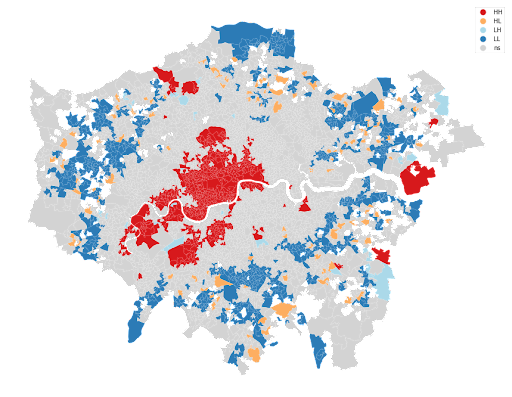
\includegraphics[width=0.65\textwidth]{2/figures/esda.png}
			\caption[Análisis Exploratorio de Datos Espaciales (ESDA)]{Análisis Exploratorio de Datos Espaciales (ESDA).\\
			Fuente: \cite{bk_haining2003spdat}. \citetitle{bk_haining2003spdat}. (p. 181)}
			\label{2:fig10}
		\end{center}
	\end{figure}
		

	\item \textbf{Modelos de Análisis Espacial}:para estimar y modelar el semivariograma, se presentan modelos de análisis espacial, como kriging con datos gaussianos que se muestra en la Figura 25. Esto es particularmente útil para datos de superficies continuos. \parencite{bk_haining2003spdat}
	
	\begin{figure}[h]
		\begin{center}
			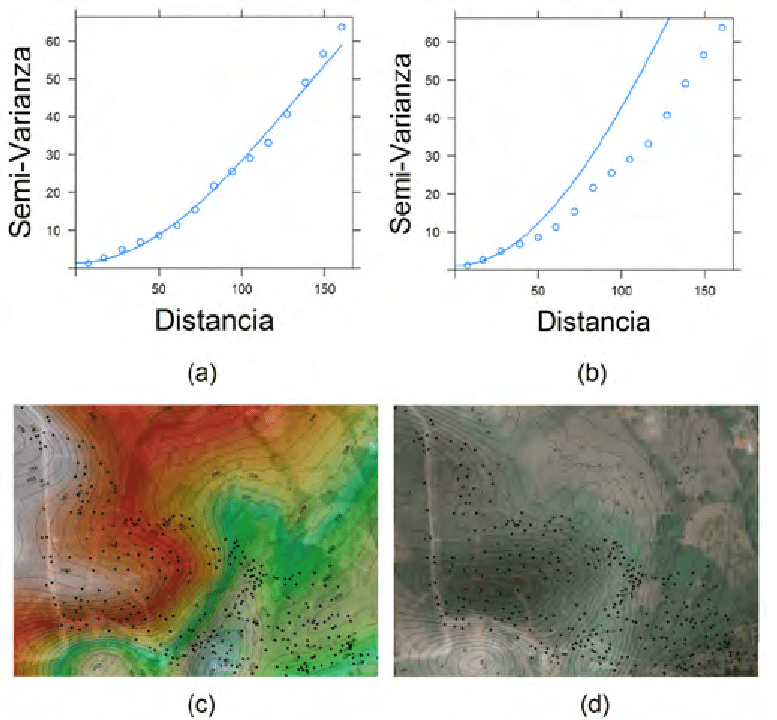
\includegraphics[width=0.70\textwidth]{2/figures/kriging.jpg}
			\caption[El modelo gaussiano isotrópico; el modelo gaussiano anisotrópico ajustado; la predicción de Kriging Simple Residual; y la varianza de Kriging Simple Residual.]{El modelo gaussiano isotrópico; el modelo gaussiano anisotrópico ajustado; la predicción de Kriging Simple Residual; y la varianza de Kriging Simple Residual.\\
			Fuente: \cite{bk_haining2003spdat}. \citetitle{bk_haining2003spdat}. (p. 352)}
			\label{2:fig11}
		\end{center}
	\end{figure}

	\item \textbf{Logistic Regression}: modela fenómenos espaciales como las relaciones entre variables espaciales y no espaciales. \parencite{bk_haining2003spdat}
	
	\begin{figure}[h]
		\begin{center}
			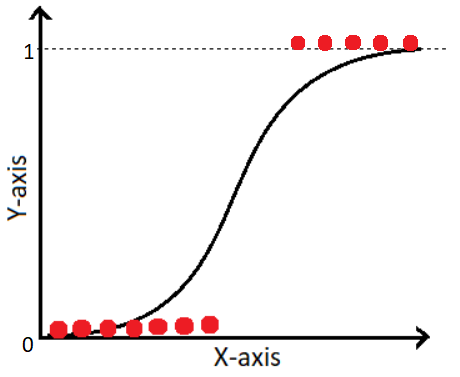
\includegraphics[width=0.70\textwidth]{2/figures/logisticregression.png}
			\caption[Regresión Logística]{Regresión Logística.\\
			Fuente: \cite{bk_haining2003spdat}. \citetitle{bk_haining2003spdat}. (p. 358)}
			\label{2:fig12}
		\end{center}
	\end{figure}
\end{itemize}
	
\subsection{Procesamiento del Lenguaje Natural}
El procesamiento del lenguaje natural (PLN) es una rama de la ciencia de la computación, la lingüística computacional, la ciencia cognitiva e la inteligencia artificial, y es un campo interdisciplinario. El objetivo es que las computadoras aprendan a hablar el lenguaje humano para que puedan realizar tareas útiles y comunicarse con las personas. El reconocimiento de voz, la comprensión del lenguaje hablado, los sistemas de diálogo, el análisis léxico y el análisis de sentimientos son solo algunas de estas tareas. \parencite{bk_deng2018deeplearningnlp}

En su libro, los autores \citeauthor{bk_deng2018deeplearningnlp} dividen el aprendizaje profundo, el racionalismo y el empiricismo en tres corrientes históricas.

\begin{itemize}
	\item \textbf{Racionalismo}: se basa en la teoría de Noam Chomsky sobre la naturaleza del lenguaje humano, desarrollada en las décadas de 1960 y 1980. Se basa en el conocimiento inherente, transmitido genéticamente y presente desde el nacimiento. La primera utilización de esta táctica se remonta a los años 50, cuando Alan Turing realizó experimentos conocidos como "las pruebas de Turing" para simular conversaciones en lenguaje natural entre un humano y una computadora con el fin de generar respuestas similares a las de una persona y evaluar así sus capacidades. Durante las décadas de 1970 y 1980, los sistemas de comprensión del lenguaje hablado y de diálogo se basaron en conjuntos de reglas creados mediante ingeniería de conocimiento experto.
	
	\item \textbf{Empirismo}: se distingue por utilizar el Aprendizaje Automático y utilizar grandes corpus de texto. Esta perspectiva sostiene que el cerebro humano funciona mediante asociaciones, reconocimiento de patrones y generalizaciones. Los modelos de traducción de IBM y el Modelo Oculto de Markov (HMM) son ejemplos de esto.
	
	\item \textbf{Aprendizaje Profundo}: resuelve los problemas de lenguaje natural que el Aprendizaje Automático tradicional no puede resolver, particularmente cuando se trata de grandes cantidades de datos. Debido a su capacidad para personalizar su arquitectura a través de múltiples capas e hiperparámetros, que permite un entrenamiento extenso, las redes neuronales artificiales son las más utilizadas. Sin embargo, a pesar de sus ventajas, tienen limitaciones, como la alta necesidad de capacidad computacional, la falta de precisión para obtener resultados estadísticos sobresalientes y la dificultad para comprender relaciones interoracionales, como frases o palabras progresivas dentro de una oración.
\end{itemize}

Los modelos mencionados anteriormente incluyen las Redes Neuronales Convolucionales (CNN) y las Redes Neuronales Recurrentes (RNN), que son algunas de las técnicas de aprendizaje profundo que se utilizan actualmente para resolver problemas de lenguaje natural. A continuación se describen algunos de los más comunes, junto con las principales características y diferencias de los ejemplos ya mencionados.

\begin{itemize}
	\item \textbf{Redes Neuronales Convolucionales}: Las técnicas de minería de datos abordan todos los conceptos y categorías de redes neuronales artificiales, incluidos los mencionados anteriormente. Hoy en día, el procesamiento de imágenes, que incluye problemas de clasificación y visión por computadora, es una de sus aplicaciones más relevantes. El proyecto de Yann LeCun, ImageNet, utiliza el reconocimiento de objetos en imágenes.
	
	Estas redes también se utilizan para clasificar textos. Ronan Collobert y Jason Weston modificaron la arquitectura y los parámetros internos de las CNN para usarlas en tareas de procesamiento de lenguaje natural. La Figura \ref{2:fig40} muestra la estructura de una CNN para problemas de procesamiento de información natural. \parencite{bk_kamath2019deeplearning_nlp_sr}
	\begin{figure}[!ht]
		\begin{center}
			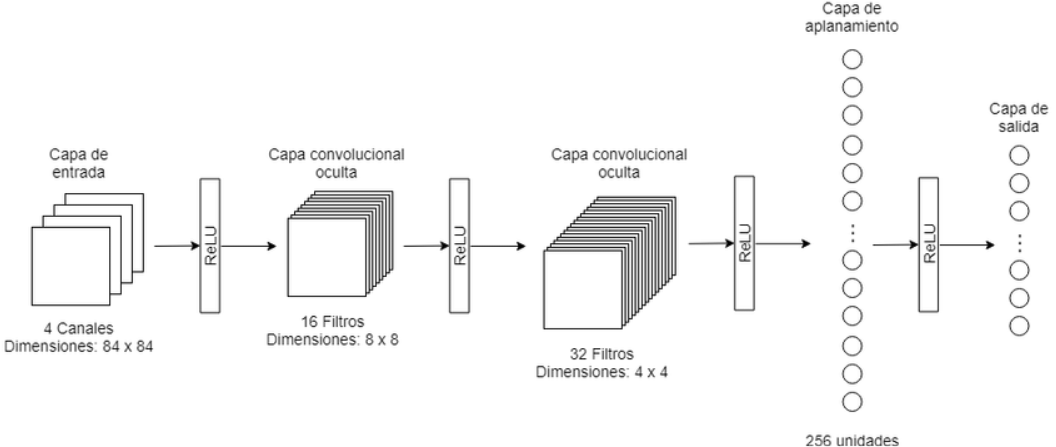
\includegraphics[width=0.95\textwidth]{2/figures/cnn_nlp.png}
			\caption[Arquitectura de un modelo CNN]{Arquitectura de un modelo CNN.\\
			Fuente: \cite{tec_kim2014convolutional}. \citetitle{tec_kim2014convolutional}. (p. 1747)}
			\label{2:fig40}
		\end{center}
	\end{figure}
	
	Debido a que se mueven a través de matrices en dos dimensiones, las convoluciones de imágenes suelen ser bidimensionales (2D). Sin embargo, debido a que están conformadas por vectores y aprenden patrones en la dimensión de secuencia, las convoluciones unidimensionales (1D) son extremadamente útiles para las series de tiempo y las operaciones de lenguaje natural. La Figura \ref{2:fig41} compara ambos tipos de convolución según el tamaño de dimensión. \parencite{bk_rao2019nlp_pytorch}

	\begin{figure}[!ht]
		\begin{center}
			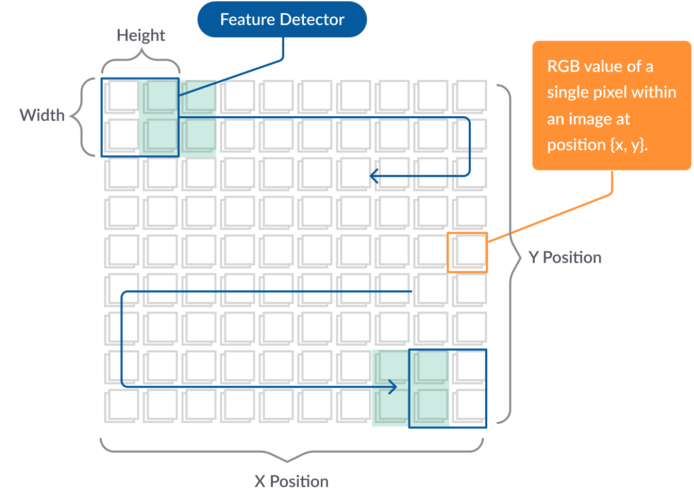
\includegraphics[width=0.95\textwidth]{2/figures/2D-convolutional-example.png}
			\caption[Diferentes dimensiones de convoluciones]{Diferentes dimensiones de convoluciones.\\
			Fuente: \cite{tec_missinglink_conv1d}. \citetitle{tec_missinglink_conv1d}.}
			\label{2:fig41}
		\end{center}
	\end{figure}

	En la Figura 28, el código final está representado por un vector, un nodo de convolución de máximo 2 bloques que cubre toda la frase con un paso de 1 bloque.

 	El proceso de arquitectura CNN generalmente se basa en los problemas de clasificación de texto considerados en esta investigación y algunas priorizaciones relacionadas con el contenido del texto.

 	La ID genérica es la creación de los vectores de los códigos Mots para la matriz de entidad genérica, que es la misma que los unidimensionales para los mapas de características genéricos de la siguiente entrada. Para generar vectores nuevos y consistentes después de cada resultado, se reagrupan según la función de los criterios utilizados (por ejemplo, máximo, mínimo, mes, etc.) y luego se vinculan al valor.

	\item \textbf{Redes Neuronales Recurrentes}: los tipos de redes neuronales más conocidos también hablaron brevemente sobre este tipo de redes. Incluso en series de tiempo, las RNN son muy utilizadas porque los datos son secuencias, es decir, una colección ordenada de elementos. En el lenguaje humano, donde los fonemas son secuencias de palabras, se puede usar un elemento dependiente para predecir la siguiente palabra en una oración dada. En este ejemplo, las palabras previas \parencite{bk_rao2019nlp_pytorch}. Los motores de búsqueda en navegadores o sitios web, traductores, entre otros, son ejemplos de estos casos de uso más comunes.
	
	\item \textbf{Modelo Secuencia a Secuencia}: una técnica común en la traducción es la generación de lenguaje natural (NLG), que se basa en dos capas LSTM. La primera capa transforma la oración de entrada en un "vector de pensamiento", mientras que la segunda capa decodifica la respuesta, como se ve en la Figura \ref{2:fig46}. Según \parencite{bk_deng2018deeplearningnlp}.
	
	\begin{figure}[!ht]
		\begin{center}
			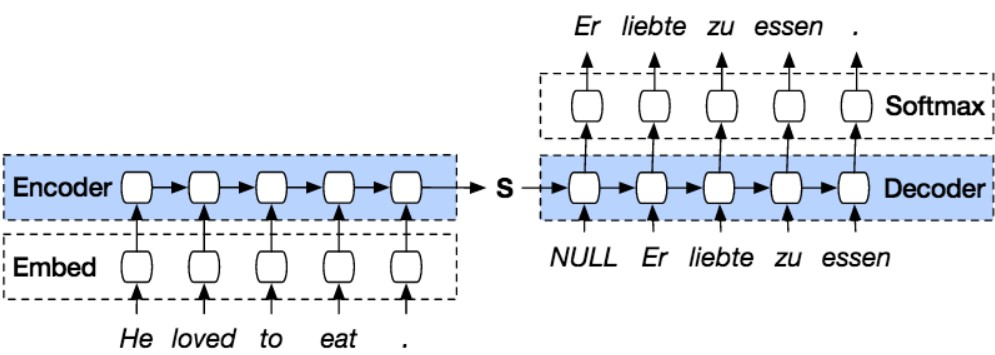
\includegraphics[width=0.67\textwidth]{2/figures/encoder-decoder.jpg}
			\caption[Arquitectura de un modelo Seq2seq]{Arquitectura de un modelo Seq2seq.\\
			Fuente: \cite{tec_kostadinov2019seq2seq}. \citetitle{tec_kostadinov2019seq2seq}.}
			\label{2:fig46}
		\end{center}
	\end{figure}	
\end{itemize}

Dado que los modelos de aprendizaje automático o profundo no pueden incluir el texto en su estado original sin limpiarlo previamente, estos modelos requieren un preprocesamiento del contenido textual. La biblioteca Natural Language Toolkit (NLTK) de Python facilita la modelización y el trabajo con texto. Sus funciones incluyen dividir el texto en oraciones, tokenizar, eliminar puntos y palabras de parada, reducir palabras a su forma raíz y convertir palabras a su forma base o diccionario. \parencite{bk_brownlee2017deeplearning_nlp}

\subsection{Redes Generativas Antagónicas}

Las redes generadoras y discriminadoras son las dos redes que compiten entre sí en las Generative Adversarial Networks (GAN). El discriminador determina si los datos son reales o generados por el generador, mientras que la función del generador es producir nuevos datos que se asemejen al conjunto de datos de entrenamiento. \parencite{tec_goodfellow2014gan}

En este juego de suma cero, quien gana pierde. El generador tiene un alto error si el discriminador clasifica correctamente los datos generados, y viceversa. Debido a que dos tipos de redes trabajan juntos, el proceso de entrenamiento es esencial. \parencite{tec_goodfellow2014gan}

Las GAN se utilizan principalmente para producir datos que se asemejan a los de entrada. Esto puede ser simplemente para generar nuevos datos o para aumentar el tamaño de un conjunto de datos existente para entrenar otra red neuronal. \parencite{tec_goodfellow2014gan}

\subsubsection{Arquitectura de las GAN}

La Figura 30 muestra la relación entre el generador y el discriminador en una GAN. El discriminador debe determinar la procedencia de cada imagen que recibe, que puede provenir de un generador o de un conjunto de datos. Mientras tanto, los valores aleatorios se convierten en imágenes que el discriminador reconoce como pertenecientes al conjunto de datos a través del generador. \parencite{tec_goodfellow2014gan}

\begin{figure}[!ht]
	\begin{center}
		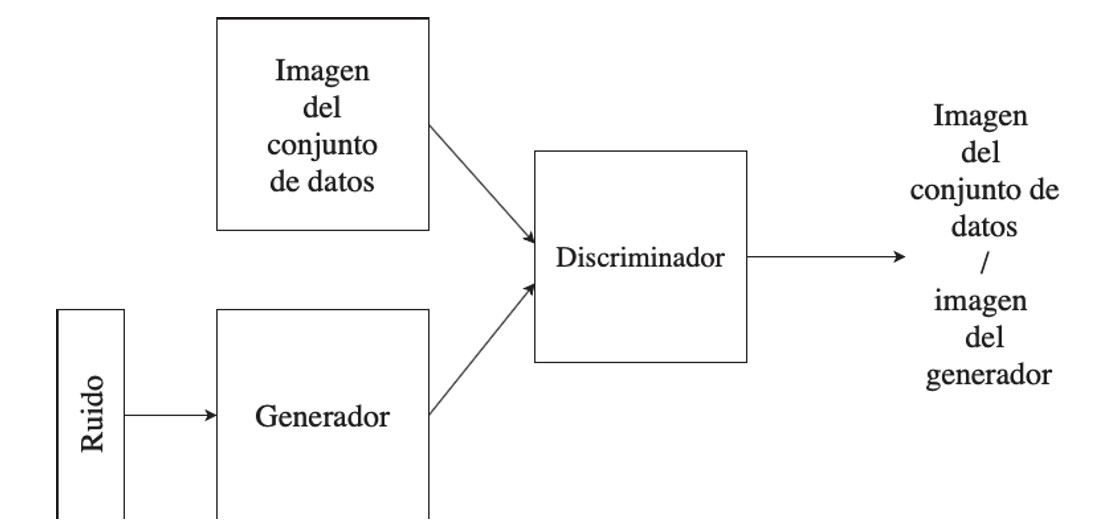
\includegraphics[width=0.75\textwidth]{2/figures/redgan.jpg}
		\caption[Red Generativa Antagónica de Imágenes]{Red Generativa Antagónica de Imágenes.\\
		Fuente: \cite{tec_goodfellow2014gan}. \citetitle{tec_goodfellow2014gan}.}
		\label{2:fig47}
	\end{center}
\end{figure}

El uso de GANs es amplia y no se limita a un tipo de datos específico. La Figura 31 muestra una GAN con un generador y un discriminador de dos capas. En el generador, cada capa es gradualmente más grande, mientras que en el discriminador, cada capa se vuelve más pequeña hasta que se encuentra una neurona en la última capa. \parencite{tec_goodfellow2014gan}

\begin{figure}[!ht]
	\begin{center}
		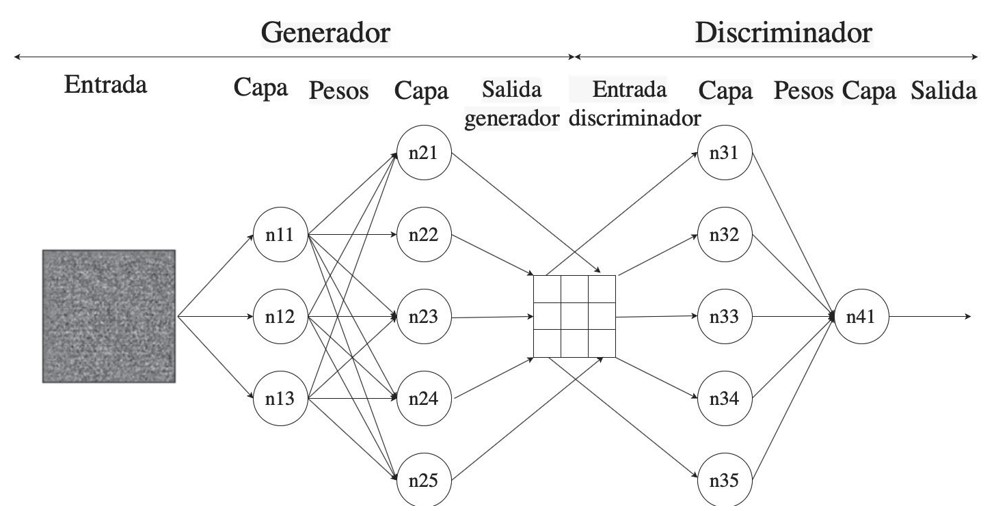
\includegraphics[width=0.75\textwidth]{2/figures/redgan2.jpg}
		\caption[Red Generativa Antagónica de Imágenes]{Red Generativa Antagónica de Imágenes.\\
		Fuente: \cite{tec_goodfellow2014gan}. \citetitle{tec_goodfellow2014gan}.}
		\label{2:fig48}
	\end{center}
\end{figure}

Como se muestra en la Figura 32 con imágenes en blanco y negro, la entrada del generador es una distribución aleatoria gaussiana. Su salida es comparable a la del conjunto de datos, y la capa de salida debe tener suficientes neuronas dispuestas de manera adecuada para producir datos con la misma estructura que el conjunto de datos original, ya sea imágenes, audio o cualquier otro tipo de datos. Por ejemplo, si se quieren imágenes de 20 x 20 píxeles, el generador debe producir 400 neuronas. Cada capa del generador es más grande que la anterior y generalmente utiliza la activación Selu, excepto la capa final, que utiliza Sigmoide. \parencite{tec_goodfellow2014gan}

\begin{figure}[!ht]
	\begin{center}
		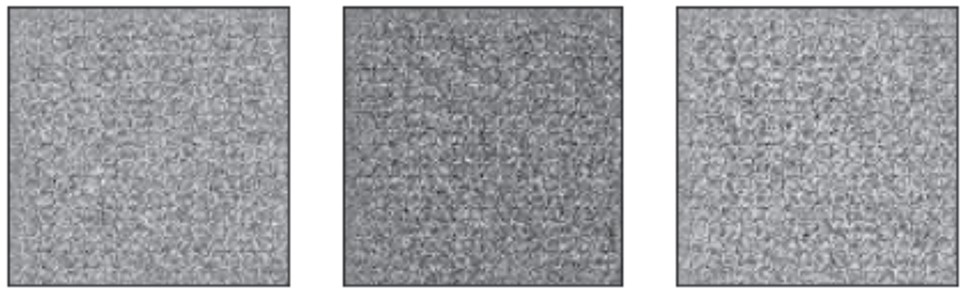
\includegraphics[width=0.75\textwidth]{2/figures/redgan3.jpg}
		\caption[Imágenes de Ruido Gaussiano]{Imágenes de Ruido Gaussiano.\\
		Fuente: \cite{tec_goodfellow2014gan}. \citetitle{tec_goodfellow2014gan}.}
		\label{2:fig49}
	\end{center}
\end{figure}

Los datos del conjunto de datos o los creados por el generador son la entrada del discriminador. Su salida consiste en una neurona con un solo valor numérico que intenta determinar si la entrada proviene del generador o del conjunto de datos. Por lo general, cada capa del discriminador contiene menos neuronas hasta que solo queda una neurona en la capa más alta. \parencite{tec_goodfellow2014gan}

\subsubsection{Entrenamiento de las GAN}

En el primer paso del proceso, el discriminador recibe capacitación para diferenciar entre imágenes reales y imágenes creadas por el generador. El generador se entrena para crear imágenes en el segundo paso, pero los pesos del discriminador no se actualizan en este caso. Las imágenes generadas se etiquetan como reales y el generador ajusta sus pesos para que el discriminador piense que son reales. Esto mejora su capacidad para generar imágenes más parecidas al conjunto de datos original mediante la retropropagación del gradiente. \parencite{bk_geron2019machilear}

Hasta que el generador produzca resultados satisfactorios, estos pasos se repiten. El discriminador se entrena con las imágenes recién generadas y luego se enseña al generador con lo que el discriminador ha aprendido. \parencite{bk_geron2019machilear}

\subsubsection{Dificultades del entrenamiento de las GAN}

El juego de suma cero en las GAN significa que cuanto menor sea el error de uno de los elementos, mayor será el error del otro. Cuando ninguna de las dos redes cambia su estrategia, se alcanza un estado de equilibrio de Nash. Este equilibrio se alcanza cuando el generador crea imágenes perfectamente realistas y el discriminador intenta clasificarlas con una probabilidad del 50\% como generadas o del conjunto de datos. Es necesario aplicar la técnica de prueba y error durante el entrenamiento de una GAN porque no se puede garantizar que se llegue a este equilibrio. \parencite{bk_geron2019machilear}

Cuando el conjunto de datos incluye varias clases, como diferentes tipos de mascotas (gatos, perros y conejos), el entrenamiento de una GAN se vuelve más difícil. Aunque el objetivo del discriminador sigue siendo distinguir entre imágenes reales y generadas, puede haber una clase en la que el generador produzca más imágenes que el discriminador clasifique como reales, mientras que en otras clases puede haber deficiencias. Por ejemplo, el generador puede ser muy hábil en la creación de imágenes de perros, pero no lo es en otras categorías. Esto puede llevar al generador a producir más imágenes de perros y olvidarse de cómo producir imágenes de otras clases. Al recibir principalmente imágenes de perros, el discriminador puede fallar en clasificar correctamente las imágenes de otras clases. \parencite{bk_geron2019machilear}

\subsection{Generación de Imágenes}

En los últimos años, ha habido una notable evolución en la generación de imágenes a través de la inteligencia artificial, impulsada por dos modelos generativos importantes: los autocodificadores variacionales y las redes generativas antagónicas, particularmente las que utilizan capas convolucionales. Aunque existen otras técnicas para generar imágenes no relacionadas con la IA, como las utilizadas en cine o videojuegos, se utiliza el término "imágenes generadas por ordenador" o CGI en inglés para estos fines. A pesar de que este término incluye una variedad de técnicas, en su mayoría implica modelar objetos en tres dimensiones, aplicar texturas y renderizarlos en dos dimensiones. \parencite{tec_kingma2019variat}

DCGAN, o GAN con capas convolucionales, es una herramienta común para la generación de imágenes. Como las GAN convencionales, tiene un generador y un discriminador. La Figura 33 muestra la estructura típica de una DCGAN, que utiliza una capa inicial de tres neuronas, seguida de tres capas de normalización y convolución transpuesta, produciendo una imagen a color. El discriminador, por otro lado, utiliza dos capas de convolución, dos capas de reducción y dos capas totalmente conectadas. \parencite{tec_kingma2019variat}

\begin{figure}[!ht]
	\begin{center}
		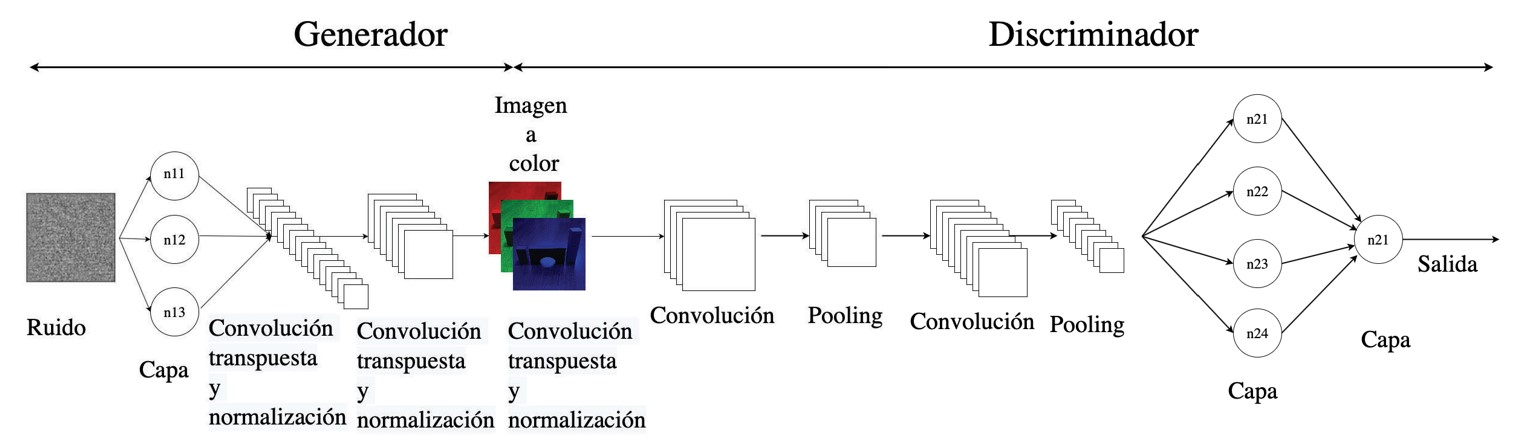
\includegraphics[width=1\textwidth]{2/figures/genimagenes.jpg}
		\caption[Arquitectura de Red Generativa Antagónica con Capas Convolucionales (DCGAN)]{Arquitectura de Red Generativa Antagónica con Capas Convolucionales (DCGAN).\\
		Fuente: \cite{tec_kingma2019variat}. \citetitle{tec_kingma2019variat}.}
		\label{2:fig50}
	\end{center}
\end{figure}

La entrada de ruido del generador se procesa a través de capas de normalización y convolución transpuesta para crear la imagen deseada. La entrada del discriminador conecta la salida del generador, que clasifica las imágenes como generadas o reales. El discriminador generalmente se compone de capas convolucionales y redes neuronales, con una sola neurona de salida con activación Sigmoide. \parencite{tec_kingma2019variat}

Los autocodificadores variacionales (VAE), que tienen similitudes con las GAN, son otra técnica común para generar imágenes. Los VAE consisten en un codificador y un decodificador y tienen como objetivo reconstruir las entradas de la red. El codificador reduce gradualmente la dimensionalidad de los datos hasta obtener una representación latente, que el decodificador reconstruye posteriormente. Los VAE pueden producir datos similares a los de entrenamiento y aplicar aleatoriedad para generar nuevas muestras. \parencite{tec_kingma2013bayes}

La interpolación de datos es otra aplicación de los autocodificadores y los VAE; en este caso, la representación latente de dos datos se combina ponderadamente para generar nuevas muestras. Interpolar entre dos muestras ya existentes permite la creación de nuevas instancias de datos. \parencite{tec_kingma2013bayes}

\newpage